% This is LLNCS.DEM the demonstration file of
% the LaTeX macro package from Springer-Verlag
% for Lecture Notes in Computer Science,
% version 2.3 for LaTeX2e
%
\documentclass{llncs}
%
\usepackage{makeidx}  % allows for indexgeneration
\usepackage{listings}
\usepackage[usenames,dvipsnames]{color}
\usepackage[hyphens]{url}
\usepackage{hyperref}
\usepackage{graphicx}
\usepackage{booktabs} 
\usepackage{url} 
%\usepackage{hyperref}

\setlength{\unitlength}{1mm}

\lstdefinelanguage{JavaScript} {
    morekeywords={
        break,const,continue,delete,do,while,export,for,in,function,
        if,else,import,in,instanceOf,label,let,new,return,switch,this,
        throw,try,catch,typeof,var,void,with,yield
    },
    sensitive=false,
    morecomment=[l]{//},
    morecomment=[s]{/*}{*/},
    morestring=[b]",
    morestring=[d]'
}

% Command for listings to highlight special lines
\definecolor{LightGray}{gray}{0.8}
\newcommand{\hilight}{\makebox[0pt][l]{\color{LightGray}\rule[-4pt]{0.7\linewidth}{14pt}}}

% Command for defining a todo on the right margin
\newcommand{\todo}[1]{\marginpar{\textcolor{red}{\\#1}}}

% for tables
\newcommand{\ra}[1]{\renewcommand{\arraystretch}{#1}}

\lstset{
    language=JavaScript,
    escapechar=\%,
    captionpos=b,
    frame=tb,
    framesep=5pt,
    breaklines=true,
    basicstyle=\footnotesize\ttfamily,
    showstringspaces=false,
    keywordstyle=\ttfamily\bfseries\color{CadetBlue},
    identifierstyle=\ttfamily,
    stringstyle=\ttfamily\color{OliveGreen},
    commentstyle=\color{Gray},
    rulecolor=\color{Gray},
    xleftmargin=5pt,
    xrightmargin=5pt,
    aboveskip=\bigskipamount,
    belowskip=\bigskipamount
}

%
\begin{document}

\frontmatter          % for the preliminaries
\pagestyle{headings}  % switches on printing of running heads

\mainmatter              % start of the contributions

\title{Implementing OAuth in HPI IP}
\titlerunning{OAuth and the HPI IP} 
\author{Richard Metzler\\
	\email{r.metzler@paadee.com} 
}
\authorrunning{Metzler} 
\institute{ Hasso-Plattner-Institut\\
			Universit\"at Potsdam \\
			\url{http://www.hpi.uni-potsdam.de/}
		}

\maketitle              % typeset the title of the contribution

\begin{abstract}
Today people are using many different internet services per day. It is hard for users to remember different usernames and passwords for every service they use, so they often reuse the same username and password on different sites. This is a security issue that protocols like OpenID and OAuth try to solve. By creating a single online identity and allowing third party services to authenticate users through them, identity provider are able to solve security issues and enable single sign-on (SSO) above different websites.

By adding an OAuth service provider to the existing HPI Identity Provider we enable third party services to authorize users via OAuth and manage the user's online identities through a newly created RESTful API.
\end{abstract}
\section{Introduction }
\label{sec:intro}

Every day people use many different internet websites for their online activities. While some of these websites are used by only a few to several thousend people, some other websites like webbased email programms or social networking websites are visited by millions of users on a daily basis. Google's GMail online email application, Facebook and Twitter aim to become the center of our online activities and therefor the single provider of our online identity. One way for them to achieve this is to enable third party sites to allow users to sign up and log in with accounts from the identity provider. This is possible through online identity protocols like OpenID and OAuth that are able to authenticate a user and redirect him back to the third party website.

For users this feature enables a more secure and better online experience as they are not required to register with username and password at every website they want to try out. For the third party service this often means that their sign-up conversion rate can dramatically increase which often has direct influence on their economic success.

% Outline
In this paper we describe the OAuth 1.0a protocol. Then we describe our proposed privacy service that is granted access to the HPI identity provider via OAuth. We explain the changes we made in order to enable OAuth in the HPI-IP and how the API works.

% What is ...?
% Motivation & Goals
% Outline

\subsection{The OAuth Protocol}

\textbf{OAuth} is an open protocol to allow secure API
authorization in a simple and standard method from desktop and web
applications. [OAuth-spec] It enables \textbf{users} to
authenticate and authorize 3rd party applications called
\textbf{OAuth consumers} to access data that is associated with a
\textbf{restricted resource} managed by the
\textbf{service provider}.

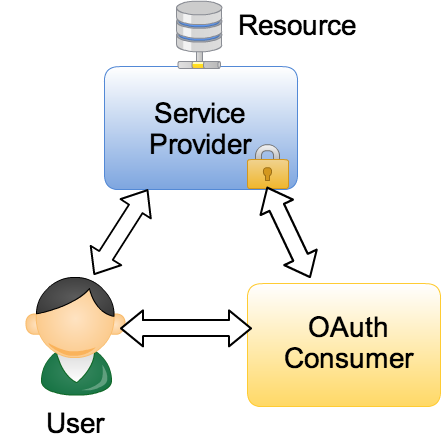
\includegraphics{../HPI-IP-OAuth/raw/master/OAuth.png}\\Image: The
three different parties in OAuth protocol. The user owns the
restricted resource and can grant access to it.

In order to authenticate an user and enabling authorization an
OAuth consumer has to be registered at the service provider
beforehand. Through registration the service provider obtains a
dedicated consumer key \& secret pair that is used for
authenticating the service whenever user access is requested. This
is an significant difference towards the OpenID protocol where
identity provider and relying party don't need to know each other
and the authentification is done decentral.

\subsubsection{OAuth Dance}

When a user wants to authenticate a webservice via OAuth the
\textbf{OAuth authentication flow} (commonly referred to as the
OAuth dance) is executed.

The following description is a simplified OAuth description as
details important for securing the authorization flow and protect
it from replay attacks like the \emph{signature method} and the
\emph{nonce} are ommitted. The description is first and foremost
meant to provide a general understanding of the OAuth
authentication flow as an full description is beyond the scope of
this paper.

The authentication flow is started by the user clicking on a
special link on the website of the OAuth consumer. The consumer
uses his consumer key and secret to request an
\textbf{unauthorized OAuth request token} and \textbf{secret} from
the service provider. This OAuth token is used to identify the
authentication context for the user.

After obtaining the request token, the user is redirected from the
consumer to the service provider. Thereby the request token is
appended to the URL. The user is authenticated and can now
authorize the consumer. After the user granted access to the
restricted resource the service provider directs the user's web
agent back to the consumer. A \emph{verifier} is appended to the
callback url.

When the user returns to the consumer the consumer uses request
token and verifier to request an \textbf{access token} and the
associated secret from the service provider. The service provider
exchanges the request token for the access token thereby granting
access to the user's resource(s) as long as the token is valid.

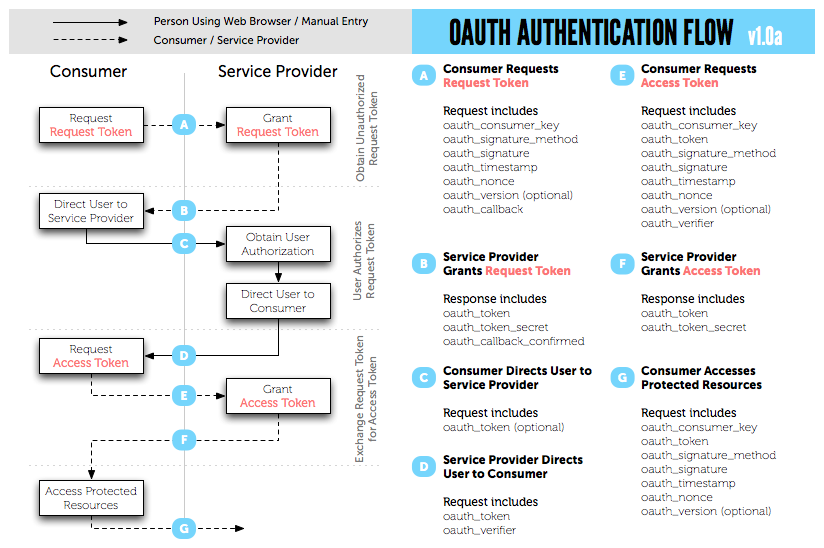
\includegraphics{../oauth_diagram.png}\\source:
\href{http://dev.twitter.com/pages/auth}{http://dev.twitter.com/pages/auth}

\section{OAuth Privacy EMail Service for HPIIP}

One main feature of the HPIIP is to act as an
\textbf{identity provider} and issue \textbf{IdentityCards}. These
Identity Cards can be used by the user to sign up to a
\textbf{relying party}, allowing the relying party requests
associated attribute values from the identity provider. These
attributes could be something like the name, home address or the
email address of the user.

In order to verify email addresses of new signed up users services
often send an email with a verification link. The user has to click
this link to verify that he signed up with a valid email address
and the user actually owns it.

Often an user only wants to try out a new service but want to
ensure his privacy and don't want to provide his real email address
in fear of SPAM from the service. Our proposed OAuth example
service should be able to change the associated email address value
of an identity card when it is authorized by the user.

To grant access to the identity card the user authorize the Privacy
EMail Service by clicking on a ``Log in to HPI IP'' button on the
Privacy EMail Service site. The service then acts as a OAuth
consumer, redirecting the user's browser to the HPI IP website to
login. The user then can grant access of the identity cards to the
consumer.

The service changes the value of the email address in an issued
identity card every 10 minutes to a temporary valid email address
the service has control of. Whenever a user sign up to a relying
party with his identity card, the relying party request the current
email address attribute from the identity provider and sends an
email. The identity provider will return the temporary email
adress. Because the OAuth service forwards emails for 20 minutes to
the actual email address of the user and ignores emails to the
temporary address received thereafter the user will receive only
the emails from the relying party that are send in this short time
window. All emails received later are considered `SPAM' and will be
ignored.

\begin{figure}
	\centering
	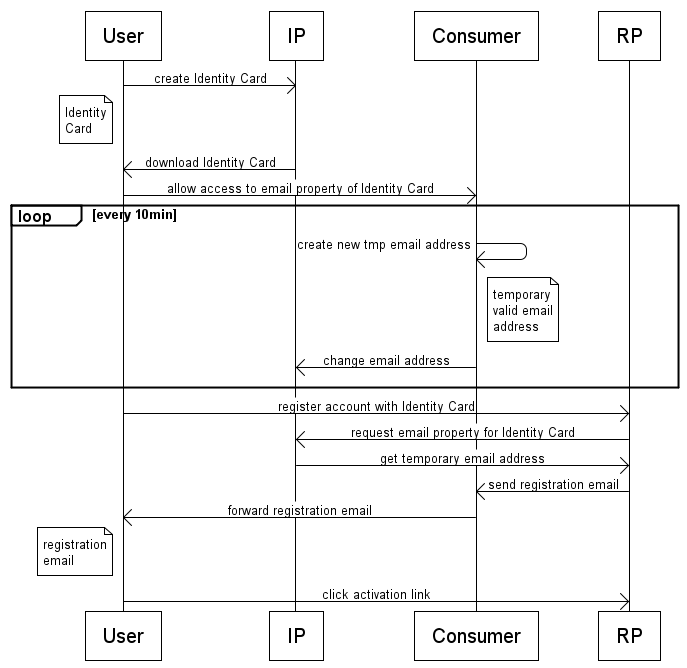
\includegraphics[width=\textwidth]{../HPI-IP-OAuth/raw/master/example-service-seq.png}
	\caption{Sequence diagram of the proposed privacy service.}  
\end{figure}


\subsection{Implementation}

Our example service has to be a webservice able to receive and send
emails. Because we were not in control of and did not want to set
up an own SMTP server we choose to use [Google AppEngine].

Google AppEngine is a \emph{Plattform as a Service} infrastructure
framework provided by Google. Developers can use Python and Java
(in fact every programming language that can be run on the Java VM)
to programm web applications for this infrastructure. Like most web
frameworks Google AppEngine also implements the
\emph{Model-View-Controller (MVC) pattern}. The framework also has
APIs to receive and send emails and start Cron jobs.

When an user clicks on the ``login with HPIIP'' at the service
application website he will be redirected to the HPI IP where he
can login and grant access to the service. After granting access he
then will be redirected back to the application and can complete
the setup. The service is now able to access the restricted
ressources in behalf of the user.

We can configure a cron job that will call a specific method
recurrently every 10 minutes to set up a new temporary email
address and use the API of the HPI IP to store it as configured by
the user. The same email address is stored by the service and
associated with the real email address of the user.

Applications running on Google AppEngine are able to receive and
send mails. When the service receives an email it looks for the
this address in the temporary email address table. If it exists the
email will be redirected to the associated actual email address of
the user.

\section{Implementing OAuth in HPI IP}

If you have to implement an OAuth consumer you can find many client
implementations in every programming language possible.
Unfortunately the same does not hold for implementing an OAuth
provider. While there are various implementations for scripting
languages (notably Ruby, Python and PHP) and even an experimental
API for using Google AppEngine as OAuth service provider \cite{gae-oauth} we have found only one
example implementation for Java. \cite{java-oauth} 

This implementation unfortunately isn't a simple to use framework
where the developer just provides the persistence layer and the web
layer and gets the logic for creating the tokens for free. It is only
an example implementation using servlets for implementing the OAuth URLs.
We tried to recreate the logic found there in the example code
using the Java Persistence API (JPA) for the persistence layer and
Apache Tapestry for the web layer. Apache Tapestry was used by the
HPI IP before.

\subsection{Implementing OAuth URLs}

OAuth defines three request endpoint URLs:

\begin{itemize}
\item
  Request Token URL - we use \emph{/oauth/request\_token}
\item
  User Authorization URL - we use \emph{/oauth/authorize}
\item
  Access Token URL - we use \emph{/oauth/access\_token}
\end{itemize}
These endpoints are required to be implemented with the Apache
Tapestry5 webframework that is used within the HPI IP.

\subsection{Request Token URL}

When the consumer sends an HTTP requests to the Request Token URL
\emph{/oauth/request\_token} there must be the following parameters
specified:

\begin{itemize}
\item
  \emph{realm}
\item
  \emph{oauth\_consumer\_key}
\item
  \emph{oauth\_signature\_method}
\item
  \emph{oauth\_callback}
\item
  \emph{oauth\_signature}
\end{itemize}
The service provider must validate the incoming OAuth message and
verify the consumer by checking his credentials against the
database. Then the service provider creates a new set of temporary
credentials and returns it in a HTTP response body using
\emph{``application/x-www-form-urlencoded''} content type.

If the request was valid the response contains the following url
encoded parameters:

\begin{itemize}
\item
  \emph{oauth\_token}
\item
  \emph{oauth\_token\_secret}
\item
  \emph{oauth\_callback\_confirmed}
\end{itemize}
This oauth token is called the \emph{request token} and it is used
to identify the OAuth authorization flow.

\subsection{User Authorization URL}

After receiving the \emph{request token} the OAuth consumer
redirects the user's web browser to the \emph{authorization url}
with the request token appended as parameter
\textbf{oauth\_token}.

The provider has to verify the identity of the user and then ask to
authorize the requested access. Therefor the OAuth provider should
display informations about the client based on the request token
(like the OAuth client's name, url or logo) for the user to
verify.

To prevent repeated authorization attempts the provider has to
delete or mark the request token as used. If the user authorize the
consumer the user's webbrowser is redirected to the consumer's
callback url and \emph{oauth\_token} and \emph{oauth\_verifier} are
appended as parameters.

\subsection{Access Token URL}

When the user is redirected to the OAuth consumer the consumer uses
the \emph{oauth\_verifier} to obtain the permanent access token. To
do this the \emph{oauth\_verifier} is added to the list of
parameters the consumer used to obtain the request token and all
parameters are appended to the access token url.

The server must verify the validity of the request. If the request
is valid and authorized the permanent token credentials are
includes as ``application/x-www-form-urlencoded'' content type with
status code 200 (OK) in the HTTP response. The parameters are

\begin{itemize}
\item
  \emph{oauth\_token}
\item
  \emph{oauth\_token\_secret}
\end{itemize}
Once the client receives and stores the token credentials it can
use it to access protected resorces on behalf of the resource
owner. To do so the consumer has to use his credentials together
with the access token credentials received.

\section{Application Programming Interface (API)}

Whenever the consumer tries to access the user's restricted
resource he has to add the OAuth protocol parameters to the request
by using the OAuth HTTP ``Authorization'' header field. The
required parameters are:

\begin{itemize}
\item
  \emph{oauth\_consumer\_key}
\item
  \emph{oauth\_token}
\item
  \emph{oauth\_signature\_method}
\item
  \emph{oauth\_timestamp}
\item
  \emph{oauth\_nonce}
\item
  \emph{oauth\_signature}
\end{itemize}
The server has to validate the authenticated request by
recalculating the request signature, ensuring that the combination
of \emph{nonce / timestamp / token} has never used before and
verify that the scope and status of the authorization as
represented by the OAuth request token is valid.

\subsection{Granularity of Rights Management}

While most existing OAuth providers (e.g. Twitter) manage rights
only at the granularity of of the access token allowing or denying
read/write access to every of the user's resources, it is often
feasible to manage rights with finer granularity. In fact this is
what we need to do in the HPI IP in order to allow users to grant
access to some relevant attributes of their identities and deny
access to others.

By this means that not only the API used by service consumers is becoming more
complex, the complexity for the user interface to manage access
rights for consumers transparently increases too. If this problem
isn't solved in the user interface it could lead to conflicts over
privacy issues like it is the case with Facebook's third party
applications.

In order to have maximum fine granularity of rights management we
decided that the user will be able to set access permissions
for each attribute seperately.

\subsection{Accessing the User's Restricted Resources}

In today's internet world there are many different technologies for
providing API access for client applications but RESTful Web Services prevail.
We decided to build the neccessary API in a restful way using URLs to name
resources, HTTP verbs for methods and HTTP response codes to signal
results. \cite{rest} This way we have to decide which resources should
be available and how they are represented.

The OAuth access token is essentially the right to access some of
the associated user's restricted resources. The OAuth client has to
query the API to find out which specific resources it can access in
behalf of the user. Therefor we need one URL endpoint that is the
same for every user. By querying it with the access token the
consumer specifies the user and gets some more information about
which resources are accessable with the provided token.

\begin{itemize}
\item
  the resource of the user who granted the access token should be
  \emph{HPIIP/api/user}
\end{itemize}
The representation of this resource in JSON should be something
like this, showing only the values that are available to the
requesting consumer:

\begin{verbatim}
{
    "user" : {
        "username" : "richard.metzler",
        "identities" : [
            {
                "main identity" : [
                    {
                        "id" : "123456",
                        "attribute" : "email",
                        "value" : "richard@...",
                        "resource" : "HPIIP/api/attribute/123456",
                        "writable" : true
                    }, ...
                ]

            }, ...
        ]
    }
}
\end{verbatim}
As you can see, the third party service is able to find out the
resource for reading and updating the email resource. Reading is
done by sending an HTTP GET request, while updating is by sending an HTTP
POST request to the \emph{HPIIP/api/attribute/\{id\}} resource and using a JSON representation as payload.
The resource is again represented in JSON format:

\begin{verbatim}
{
    "id" : "123456",
    "attribute" : "email",
    "value" : "richard@...",
    "resource" : "HPIIP/api/attribute/123456",
    "writable" : true
}
\end{verbatim}
If the client updates the value of the attribute only 
\emph{value} is required in the representation.

Whenever an OAuth consumer wants to access a resouce the OAuth
provider has to verify if the requested operation is granted to the
provided access token. It has to be denied otherwise using the HTTP
response code \textbf{401 (``Unauthorized'')}.

\subsection{Implementation}

The proposed implementation of the described API is to use
\emph{Jersey} \cite{sun-jersey}, Sun's implementation of the JAX-RS specification for RESTful Web Services. \cite{jax-rs} 
JAX-RS describes a Java API to build RESTful webservices by using
Java5 style annotations. These webservices have to run in a servlet
container like Apache Tomcat or Jetty.

Because the existing HPI IP uses the Tapestry5 webframework we had
to decide if the API and the existing application should be
deployed next to each other and use their own database bindings or
deploy it as one application in the same directory. Because we
wanted to reuse the existing database bindings we decided to use
the Tapestry-Jersey integration provided by Blue Tang
Studio. \cite{yunglin-source} \cite{yunglin-wiki}  

%\input{analysis}
%\input{conclusion}

%\newpage
%r\input{appendix}

\newpage
\bibliography{main}{}
\bibliographystyle{plain}

\end{document}
